\documentclass[12pt,a4paper]{article}
\usepackage[utf8]{inputenc}
% \usepackage[russian]{babel}
\usepackage[OT1]{fontenc}
\usepackage{color}
\usepackage{amsmath}
\usepackage{listings}
\usepackage{amsfonts}
\usepackage{amssymb}
\usepackage[pdftex]{graphicx}
\author{A.Bykov, D.Shilin, D. Nikolaeva}
\usepackage{tikz}
%tikz library includes
\usetikzlibrary[arrows]
\usetikzlibrary[automata]
\usetikzlibrary[backgrounds]
\usetikzlibrary[calc]
\usetikzlibrary[calendar]
\usetikzlibrary[chains]
\usetikzlibrary[decorations]
\usetikzlibrary[decorations.footprints]
\usetikzlibrary[decorations.fractals]
\usetikzlibrary[decorations.markings]
\usetikzlibrary[decorations.pathmorphing]
\usetikzlibrary[decorations.pathreplacing]
\usetikzlibrary[decorations.shapes]
\usetikzlibrary[decorations.text]
\usetikzlibrary[er]
\usetikzlibrary[fadings]
\usetikzlibrary[fit]
\usetikzlibrary[folding]
\usetikzlibrary[matrix]
\usetikzlibrary[mindmap]
\usetikzlibrary[patterns]
\usetikzlibrary[petri]
%%\usetikzlibrary[placements]
\usetikzlibrary[plothandlers]
\usetikzlibrary[plotmarks]
\usetikzlibrary[positioning]
\usetikzlibrary[scopes]
\usetikzlibrary[shadows]
\usetikzlibrary[shapes.arrows]
%%\usetikzlibrary[shapes.callout]
\usetikzlibrary[shapes.gates.logic.US]
\usetikzlibrary[shapes.gates.logic.IEC]
\usetikzlibrary[shapes.geometric]
\usetikzlibrary[shapes.multipart]
\usetikzlibrary[shapes.multipart]
\usetikzlibrary[shapes.misc]
\usetikzlibrary[shapes.symbols]
\usetikzlibrary[through]
\usetikzlibrary[topaths]
\usetikzlibrary[trees]
\begin{document}
\definecolor{dkgreen}{rgb}{0,0.6,0}
\definecolor{gray}{rgb}{0.5,0.5,0.5} 
\lstset{ %
  language=Octave,                % the language of the code
  basicstyle=\footnotesize,           % the size of the fonts that are used for the code
  numbers=left,                   % where to put the line-numbers
  numberstyle=\tiny\color{gray},  % the style that is used for the line-numbers
  stepnumber=1,                   % the step between two line-numbers. If it's 1, each line 
                                  % will be numbered
  numbersep=5pt,                  % how far the line-numbers are from the code
  backgroundcolor=\color{white},      % choose the background color. You must add \usepackage{color}
  showspaces=false,               % show spaces adding particular underscores
  showstringspaces=false,         % underline spaces within strings
  showtabs=false,                 % show tabs within strings adding particular underscores
  frame=single,                   % adds a frame around the code
  rulecolor=\color{black},        % if not set, the frame-color may be changed on line-breaks within not-black text (e.g. comments (green here))
  tabsize=2,                      % sets default tabsize to 2 spaces
  captionpos=b,                   % sets the caption-position to bottom
  breaklines=true,                % sets automatic line breaking
  breakatwhitespace=false,        % sets if automatic breaks should only happen at whitespace
 % title=\lstname,                   % show the filename of files included with \lstinputlisting;
                                  % also try caption instead of title
  keywordstyle=\color{blue},          % keyword style
  commentstyle=\color{dkgreen}       % comment style
}
\newcommand{\happysmile}[1]{
\begin{tikzpicture}[scale=#1/10]
  \fill[yellow] (0,0) circle (2);
  \draw (0.75,0.5) circle (0.25);
  \draw (-0.75,0.5) circle (0.25);
  \draw (1,-0.5)..controls(0,-1.5)..(-1,-0.5);
\end{tikzpicture}
}
\newcommand{\sadsmile}[1]{
\begin{tikzpicture}[scale=#1/10]
  \fill[yellow] (0,0) circle (2);
  \draw (0.75,0.5) circle (0.25);
  \draw (-0.75,0.5) circle (0.25);
  \draw (1,-1)..controls(0,-0.5)..(-1,-1);
\end{tikzpicture}
}

\newcommand{\newtitle}[2]{
\title{#1}
\author{#2}
\maketitle
\pagebreak
\tableofcontents
\pagebreak
}
\newcommand{\definition}[2]{
\underline{\textit{#1}}- #2
}
\newcommand{\code}[2]{
\lstinputlisting[caption={#2},label=DescriptiveLabel,language=sql]{#1}
}
\newtitle{Data modelling and Databases \\ [2ex] Project}{A.Bykov, D.Shilin, D.Nikolaeva}
\section{Phase 1.Creating scheme}
\subsection{Task}
We are needed to transform scheme from technical task into relations
\begin{figure}[h!]
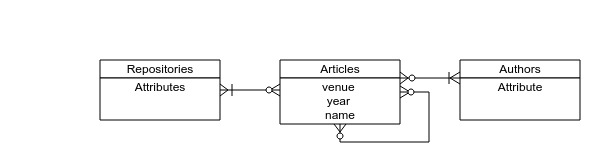
\includegraphics[scale=0.65791]{media/figure1.jpg}\\
\caption{Structure from technical task}
\end{figure}

\subsection{Relations transformations}
There are three many-to-many relations. So, we are needed to transform them all into many-to-one relations.
\subsubsection{Repositories-Articles}
A repository can contain many articles. So, many-to-many field transforms into a table Contains:\\
\begin{figure}[h!]
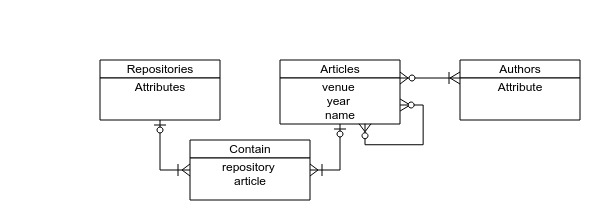
\includegraphics[scale=0.65791]{media/figure2.jpg}\\
\caption{Structure from technical task}
\end{figure}


\subsubsection{Articles-Articles}
This relation stands for referencing. In article's bibliography can be many articles. So, it transforms from Article-Article many-to-many relation into:
\begin{enumerate}
\item Article-References one-to-many
\item Reference-Article many-to-one.
\end{enumerate}
\begin{figure}[h]
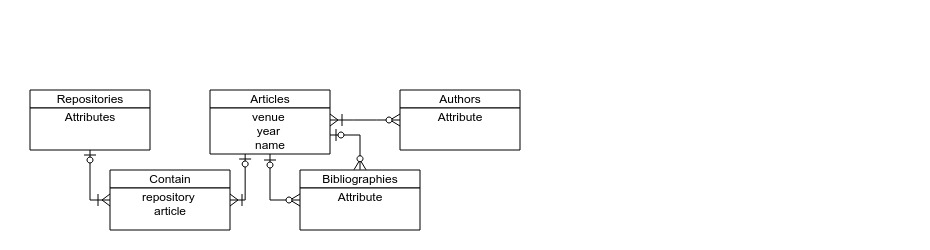
\includegraphics[scale=0.65791]{media/figure3.jpg}\\
\caption{Our structure with Bibliography}
\end{figure}

\subsubsection{Articles-Authors}
There can be many authors of one article and each author may have many publication. So, we'll transform Articles-Authors relation into:
\begin{enumerate}
\item Article-AuthorList
\item AuthorList
\end{enumerate}
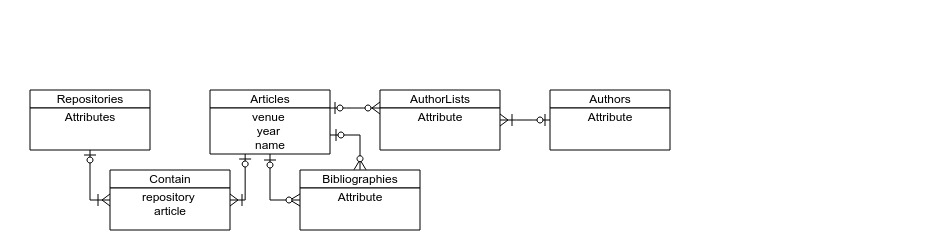
\includegraphics[scale=0.585791]{media/figure4.jpg}

\subsection{Writing relations forms}
Repositories($\underline{id}$,url,name)\\
Contain($\underline{id}$, repository\_id, article\_id)\\
Articles($\underline{id}$,venue, year, name)\\
Bibliography($\underline{id}$, article\_id, cited\_article\_id)\\
AuthorList($\underline{id}$, article\_id, author\_id)\\
Authors($\underline{id}$, name)
\section{Phase 1. Implementing scheme. PostgreSQL}
\code{src/init_db.sql}{database initialising}
\code{src/init_tables.sql}{tables initialising}
\section{Phase 1. Inserting data.}
We have python script which parses xml file into sql file with insertions.
\end{document}